\section{Exploring Thread Interleaving Space}
\label{s:design}



% In this section, we describe our approach to effectively achieve
% \textbf{Design goal 1} and \textbf{2}.


%
% Specifically, we propose a novel perspective on the thread
% interleaving exploration.
% %
% Specifically, our key idea lies in three steps:

This work focuses on how to efficiently explore the vast search space
of thread interleaving when a multi-thread input (\eg,
\texttt{sendmsg()} and \texttt{setsockopt()} in
\autoref{fig:cve-2017-17712}) is given. Our approach utilizes an
\textit{explored} thread interleaving as a seed interleaving.
%
With the seed interleaving, we explore thread interleavings of the
given input in the following three steps:
%
\begin{enumerate}[labelsep=0pt, label=\textbf{\arabic*) }]
\item \textbf{\textit{Decomposing}} an explored thread interleaving
  into segments containing a small number of instructions.
\item \textbf{\textit{Mutating}} interleavings within segments to
  generate unexplored interleavings for each segment.
\item \textbf{\textit{Recomposing}} mutated segments into whole thread
  interleaving to determine how to schedule instructions in future.
\end{enumerate}
%


In this section, we first explain our key intuition behind decomposing
an explored interleaving into \textit{interleaving
  segments}~(\autoref{ss:overview}).
%
Then, we illustrate how we define an interleaving coverage metric
based on \textit{step 1} to satisfy \textbf{Design goal
  1}~(\autoref{ss:coverage}).
%
% The coverage metric represents
% combinatorial interleavings\yj{I do not like the term, combinatorial interleaving. Is it widely used?} .
%
Lastly, we explain the mutation-based interleaving exploration method
based on \textit{step 2} and \textit{step 3} to satisfy \textbf{Design
  goal 2}~(\autoref{ss:scheduler}).
% \yj{a new thread?}  interleaving for future iterations
% (\textbf{Design goal 2})~(\autoref{ss:scheduler}).

\red{
Throughout this section, we use \autoref{fig:cve-2017-17712} as a
running example to show how a seed interleaving~(\ie,
\autoref{fig:keyidea}-(a)) is used to explore the offending
interleaving~(\ie, \autoref{fig:interleavingmutation}-(c)).
}



\subsection{Key Idea: Segmentizing thread interleaving}
\label{ss:overview}

%\begin{table}[t]
  %\centering
  %input{table/learningfrommistakes.tex}
  %\caption{Statistics provided by Shan Lu
    %\etal~\cite{learningfrommistakes}, stating the number of
    %concurrency bugs according to the number of memory accesses
    %involved in the manifestation of a concurrency bug. \yj{Do we need
      %the table?} \dr{No. we can remove this.}}
  %\label{table:learningfrommistakes}
  % \end{table}

When fuzzing for discovering concurrency bugs with an interleaving
coverage metric, the fundamental challenge is the large search space,
because the consideration of multiple memory accesses increases the
search space exponentially.
%
Therefore, this work seeks to strike the balance in the trade-off
between the bug-finding capability and the search complexity.

\PP{Segmentizing thread interleaving}
%
To reduce the search complexity, we take the classical wisdom of
problem decomposition, where the complexity of a problem exponentially
decreases as the problem size decreases.
%
Our key strategy is \textit{decomposing} the search space into small
sub-spaces. We call a sub-space \textit{interleaving segment}.
%
Each interleaving segment consists of instructions accessing 
shared memory objects.
% the same  memory objects. (\ie, conflicting instructions).
To define the size (\ie, the number of instructions) of an
interleaving segment, we use an observation from an extensive
survey~\cite{learningfrommistakes} in which 92.4\% (97 out of 105) of
concurrency bugs manifest when a bug-finding system detects specific
interleavings of \textit{at most} four memory accesses referring to
shared memory objects.
%
So, all other memory accesses beyond four accesses and their execution
orders do not meaningfully affect manifestation of a concurrency bug.
%
The observation is also applied to the example of
\autoref{fig:cve-2017-17712}. The uninitialized access bug is
triggered by the execution order of three memory accesses (\eg,
\texttt{A2}, \texttt{A4} and \texttt{B1}), while others (\eg,
\texttt{A6} and \texttt{B2}) are irrelevant to the manifestation of
the concurrency bug.
Following the observation,  we confine the size of a interleaving segment 
to contain at most four memory-accessing instructions,
which makes the problem of defining a coverage metric tractable while maintaining a strong bug-finding capability.


\PP{Example of interleaving segments}
%
\begin{figure}[t]
  \centering
  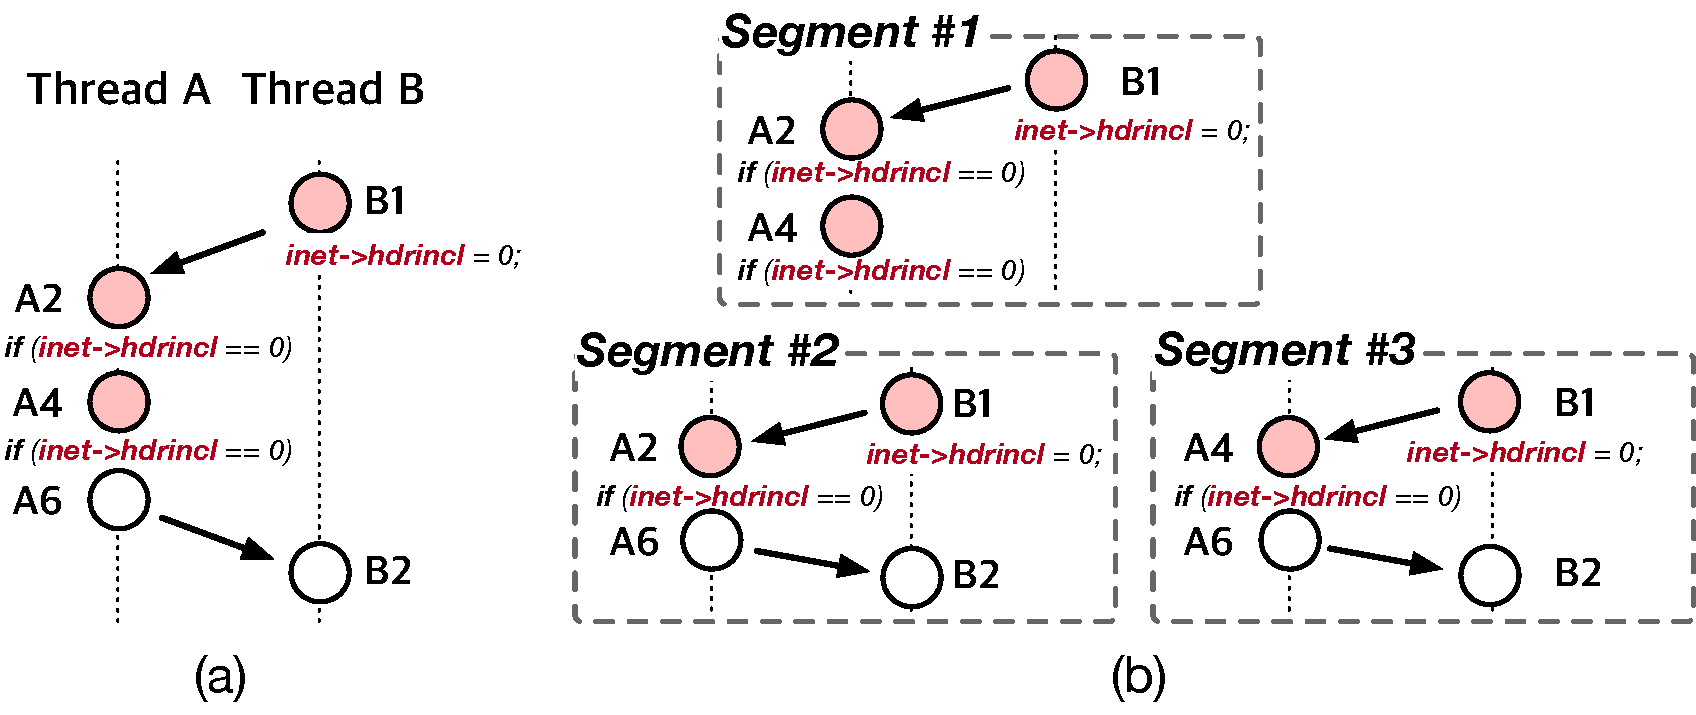
\includegraphics[width=0.99\linewidth]{fig/intuition.pdf}
  \caption{(a) A thread interleaving example of
    \autoref{fig:cve-2017-17712}, and (b) interleaving segments
    contained in (a).  Note that we intentionally omit instructions
    that do not access globally-visible memory objects.}
  \label{fig:keyidea}
\end{figure}
%
\autoref{fig:keyidea} illustrates interleaving segments from the
single execution of two system calls, where the execution scenario is
represented in \autoref{fig:keyidea}-(a).
% example shows the execution of the two system calls 
% and executed thread interleavings described in
%
Then, interleaving segments described in \autoref{fig:keyidea}-(b)
represents a part of its thread interleaving, comprised by at most
four instructions.
%
For example, \texttt{Segment \#1} represents an interleaving of three
instructions \texttt{B1}, \texttt{A2}, and \texttt{A4}, stating that
\texttt{B1} is executed before \texttt{A2} and \texttt{A4}.
%
Similarly, \texttt{Segment \#2} and \texttt{Segment \#3} describe
interleavings of (\texttt{B1}, \texttt{A2}, \texttt{A6}, and
\texttt{B2}), and (\texttt{B1}, \texttt{A4}, \texttt{A6}, and
\texttt{B2}) respectively.
How to build segments is described in \autoref{ss:coverage}.

%
%Accordingly, a fuzzer can decide that it is worth investing more
%computing power to further explore thread interleavings.
%
%Moreover, a fuzzer can infer exact execution orders that have not been
%explored, 
%
%A fuzzer therefore can systematically search thread interleavings
%directed by the inference, rather than random searching.


% Segmentizing this thread interleaving is performed in two steps.
% %
% First, we pair up two instructions that access the same mermoy object.
% %
% In \autoref{fig:keyidea}-(a), there are three pairs of such
% interleaved instructions such as
% ($\texttt{B1} \Rightarrow \texttt{A2}$) and
% ($\texttt{B1} \Rightarrow \texttt{A4}$) (accessing
% \texttt{inet->hdrincl}), and ($\texttt{A6} \Rightarrow \texttt{B2}$)
% (accessing \texttt{sk->owned}).
% %
% As we want to represent a combination of interleaving orders, the
% second step is to further combine instruction pairs into an
% interleaving segment.
% %
% Each interleaving segment is formed by combining two instruction pairs
% so that interleaving segments contain at most four instructions.
% %
% For example, we combine two instruction pairs
% ($\texttt{B1} \Rightarrow \texttt{A2}$) and
% ($\texttt{B1} \Rightarrow \texttt{A4}$) to construct \texttt{Segment
%   \#1} in which three instructions \texttt{B1}, \texttt{A2}, and
% \texttt{A4} are included.
% %
% In accordance with timestamps annotated in these instructions, we can
% arrange the instructions in \texttt{Segment \#1}.
% %
% Likewise, \texttt{Segment \#2} and \texttt{Segment \#3} are the result
% of combining $\texttt{B1} \Rightarrow \texttt{A2}$ and
% $\texttt{A6} \Rightarrow \texttt{B2}$, and
% $\texttt{B1} \Rightarrow \texttt{A4}$ and
% $\texttt{A6} \Rightarrow \texttt{B2}$ respectively.

%
% \autoref{fig:keyidea}-(a) represents the thread interleaving of the
% execution, where the uninitialized access bug does not manifest
% because \texttt{B1} is executed before \texttt{A4} (\ie,
% $(\texttt{A2} \Rightarrow \texttt{B1}) \wedge (\texttt{B1} \Rightarrow
% \texttt{A4})$ is not satisfied).
% %
% In order to track interleaving orders of a small number (\eg, four) of
% instructions, we decompose the thread interleaving into several
% interleaving segments as described in \autoref{fig:keyidea}-(b).
% %
% In these interleaving segments, \texttt{Segment \#1} contains three
% memory access operations (\ie, \texttt{A2}, \texttt{A4}, and
% \texttt{B1}), and describes interleaving orders such that \texttt{B1}
% is executed after \texttt{A2} and \texttt{A4}.
% %
% Similarly, \texttt{Segment \#2} and \texttt{Segment \#3} describes
% interleaving orders of four memory access operations, (\texttt{A2},
% \texttt{B1}, \texttt{B2}, \texttt{A6}) and (\texttt{A4}, \texttt{B1},
% \texttt{B2}, \texttt{A6}) respectively.
%

% With these interleaving segments, the fuzzer can be noticed that
% interleaving orders represented by these interelaving segments
% unlikley cause a concurrency bug.
% %
% Therefore, it is adequate for the fuzzer to search for unexplored
% interleaving segments (\eg, one that represents
% $(\texttt{A2} \Rightarrow \texttt{B1}) \wedge (\texttt{B1} \Rightarrow
% \texttt{A4})$) to maximize the chance of discovering concurrency bugs.


% %
% \dr{}
% It is worth noting that interleaving segments can be overlapped; in
% this example, \texttt{Segment \#1} and \texttt{Segment \#3} are
% overlapped over an interleaving order
% $\texttt{A4} \Rightarrow \texttt{B1}$.




\PP{Benefits of segmentizing thread interleaving}
%
Segmentizing thread interleavings provides two benefits to a fuzzer.
%
First, when defining an interleaving coverage metric, tracking
explored interleavings in each segment gives a befitting guidance to
determine whether a fuzzer further explores thread interleavings or
not.
%
% As mentioned above, most concurrency bugs manifest depending only on
% the execution order of four memory accesses.
%
Considering most concurrency bugs manifest depending on interleavings
of at most four memory accesses (which are exactly represented by
interleaving segments), if a fuzzer explores all possible
interleavings for each detected segment, it is unlikely that a fuzzer
misses a concurrency bug.
%
Accordingly, \textit{interleavings in each segment can act as an
  interleaving coverage metric, satisfying \textbf{Design goal 1}}.


% \Intcov and the form of segment graph express semantically rich
% information; it captures combinations of multiple pairs of interleaved
% instructions. At the same time, segment graphs are represented simply;
% each segment graph contains only at most four instructions.

% These two seemingly-conflicting characteristics of segment graphs
% enables the systematic exploration of thread interleaving.
% %
% In other words, it is practically impossible to thoroughly explore all
% thread interleavings of a given multi-thread input because of the
% astronomical number of possible thread interleavings.
% %
% However, it is \textit{easily possible} to throughly explore
% interleavings \textit{inside} interleaving segments due to their small
% size. More importantly, exploring inside interleaving segments is
% still enough to discover most concurrency bugs (as mentioned in
% \autoref{ss:overview}).




Second, explored interleaving segments can be used to systematically
search for interleavings in next iterations.
%
Since each interleaving segment contains only a small number of memory
accesses, a fuzzer can speculatively creates new interleavings from
explored interleavings.  Taking an example of \texttt{Segment \#1} in
\autoref{fig:keyidea}, besides execution order
($\texttt{B1} \Rightarrow \texttt{A2} \Rightarrow \texttt{A4}$)
(represented in \texttt{Segment \#1}), a fuzzer easily rearranges the
three instructions to speculate unexplored execution orders of these
instructions such as
($\texttt{A2} \Rightarrow \texttt{B1} \Rightarrow \texttt{A4}$) which
causes the uninitialized access bug if executed.  Therefore, instead
of doing a randomized \red{or heuristic} search (as in most previous
approaches), if a fuzzer figures out which of the enumerated
interleavings have not been explored, \textit{a fuzzer can
  strategically explore the search space with speculative
  interleavings, satisfying \textbf{Design goal 2}}.


% 
% \autoref{fig:hint} demonstrates how explored interleaving segments
% can be helpful for future iterations.
% %
% As illustrated in \autoref{fig:hint}, the fuzzer can derive
% \textit{unexplored} \texttt{Segment \#1*} by changing the execution
% order of \texttt{A4} and \texttt{B4} in \textit{explored}
% \texttt{Segment \#1}.
% %
% Since \texttt{Segment \#1*} satisfies
% $(\texttt{A2} \Rightarrow \texttt{B1}) \wedge (\texttt{B1} \Rightarrow
% \texttt{A4})$, the fuzzer can discover the uninitialized access bug if
% it executes thread interleaving containing \texttt{Segment \#1*}.
% %
% In addition, the fuzzer can explore multiple interleaving segments at
% a time.
% %
% Besides \texttt{Segment \#1*}, \texttt{Segment \#3*} can also be
% derived from \texttt{Segment \#3}.
% %
% Interestingly, \texttt{Segment \#1*} and \texttt{Segment \#3*} can be
% used to compose a new thread interleaving.
% %
% By executing a thread interleaving including the two derived
% interleaving segments, the fuzzer is able to quickly test a number of
% interleaving segments.
% %
% In this way, \textit{our proposed scheduler mechanism is designed to
%   quickly explore unexplored interleaving segments, and to satisfy
%   \textbf{R2}}.
% %
% \begin{figure}[t]
%   \centering
%   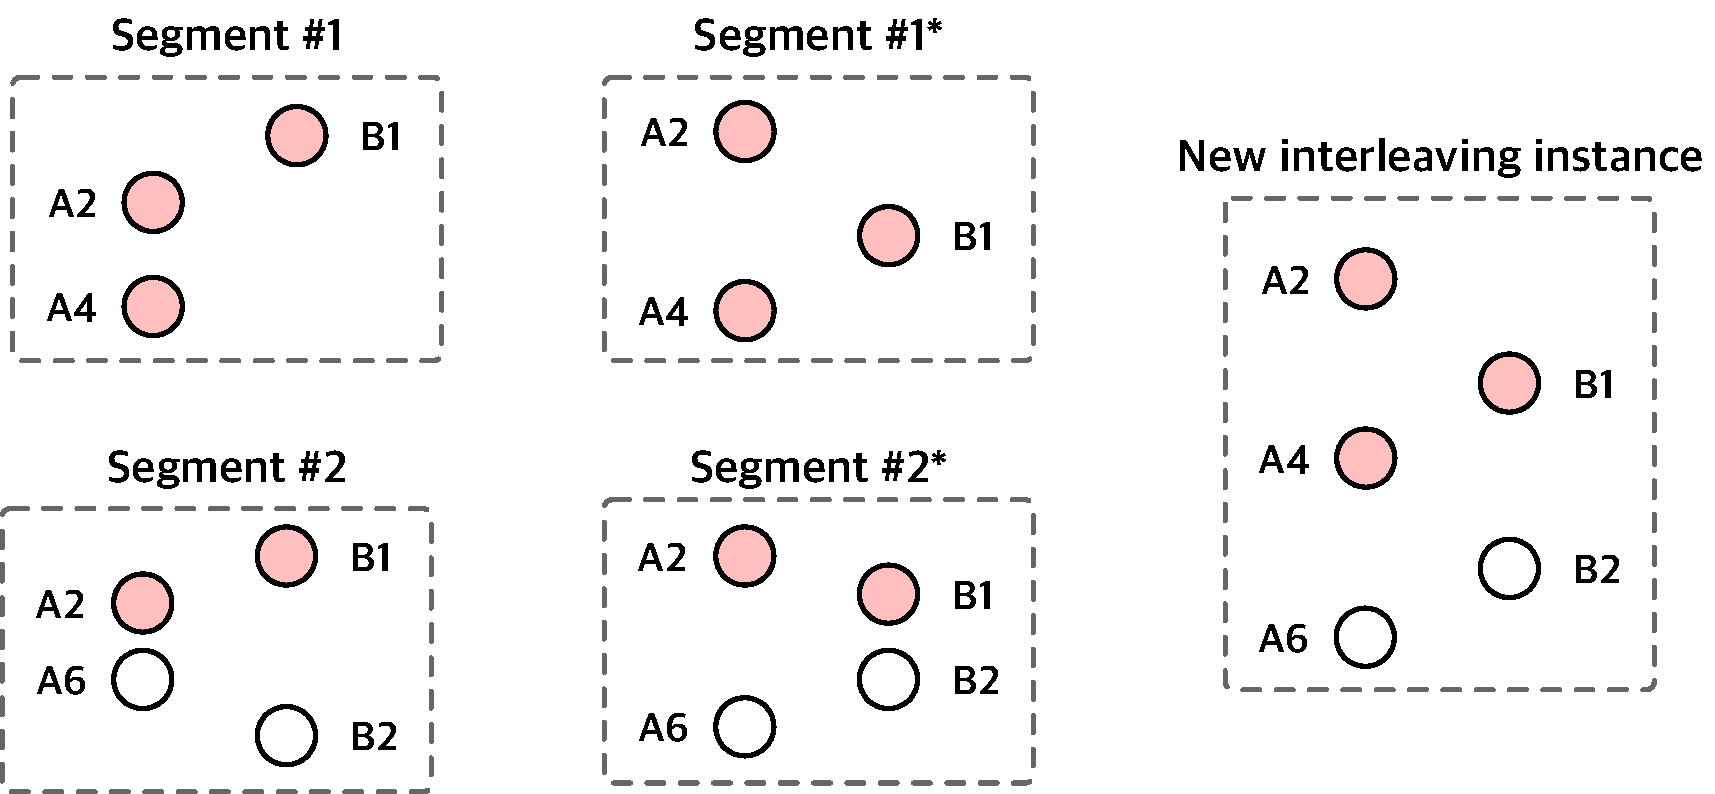
\includegraphics[width=0.9\linewidth]{fig/hint.pdf}
%   \caption{\texttt{Segment \#1} and \texttt{Segment \#3} are explored
%     interleaving segments in \autoref{fig:keyidea}.
%     %
%     From these two interleaving segments, our approach derives other
%     interleaving segments \texttt{Segment \#1*} and \texttt{\#3*}, and
%     schedules instructions to test the derived interleaving segments
%     at the same time.}
%   \label{fig:hint}
% \end{figure}
% %



\subsection{Interleaving Segment Coverage}
\label{ss:coverage}

As discussed, we \textbf{decompose} explored thread interleavings into
interleaving segments.
%
We first represent observed interleavings as a directed acyclic graph
(DAG). Then, we compute subgraphs of the DAG called \textit{segment
  graphs}, each of which represents an interleaving segment.
%
Using a set of segment graphs, we propose a novel interleaving
coverage metric called \textit{\intcov}.
%
\Intcov is a collection of explored segment graphs, designed to track
interleavings within an interleaving segment.
% , and
% to guide a fuzzer to efficiently search possible instruction
% interleavings.




% Semantically, if
% per-input \intcov is saturated, a fuzzer can confidently conclude that
% the current input unlikely causes a concurrency bug and proceed to the
% next input.
%




\PP{Graph representation of thread interleaving}
% \PP{Graph representation of interleaved instructions}
% As discussed,
% \intcov contains multiple interleaved instructions, 
% so
% \intcov cannot be presented as a single instruction interleaving 
% (e.g., $I_x \rightarrow I_y$) used in the alias coverage used in KRace.
% Instead,
In the representation of DAG,
% called an interleaving segment graph (shortly, \textit{segment
%   graph}).
%
a vertex represents a memory-accessing instruction, and an edge
represents an execution ordering between two memory-accessing
instructions. There are two types of edges,
program-order edges and interleaving-order edges.
%
A program-order edge indicates an execution order between two
memory-accessing instruction in a single thread.  Whereas, an
interleaving-order edge indicates the execution order between two
memory-accessing instructions that 1) access the same shared data, 2)
at least one of them is a write operation, and 3) are executed by
different threads.

\begin{figure}[t]
  \centering
  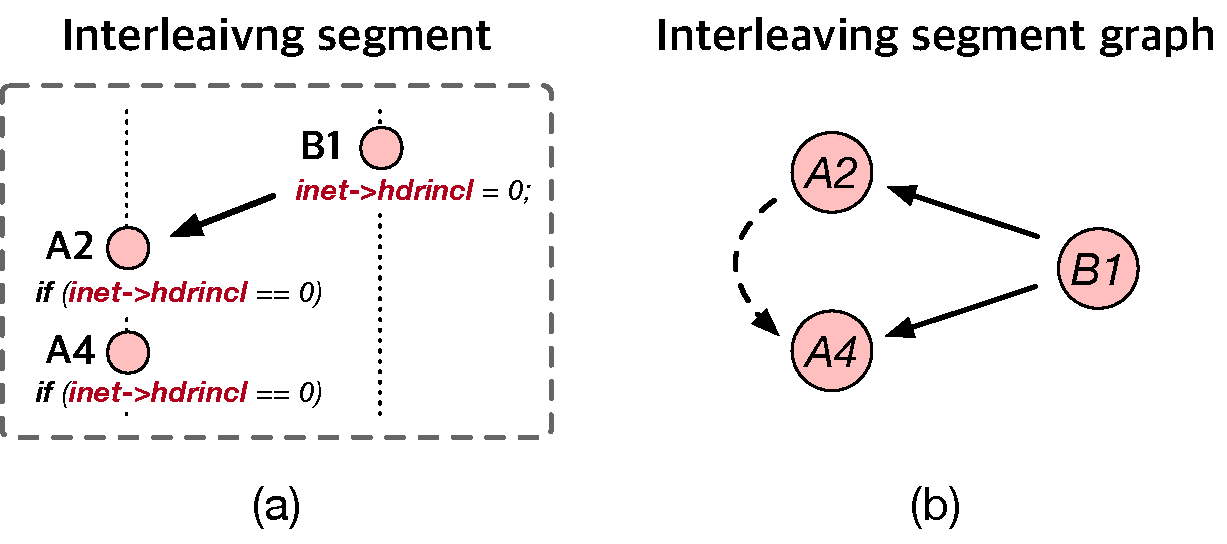
\includegraphics[width=0.8\linewidth]{fig/interleavingsegmentgraph.pdf}
  \caption{(a) Graph representation of \autoref{fig:keyidea}-(a), and
    (b) segment graph corresponding \texttt{Segment \#1} in
    \autoref{fig:keyidea}-(b). In each graph, a dotted arrow
    represents a program-order edge, and solid arrows represent
    interleaving-order edges.}
  \label{fig:interleavingsegmentgraph}
\end{figure}

%It is worth noting that a segmentgraph has two properties. First, if
%a path exists from a vertex \texttt{X} to another vertex \texttt{Y}, a
%memory access operation corresponding to \texttt{X} is executed before
%a memory access operation corresponding to \texttt{Y}.
%%
%\dr{}
%This is because edges represent orderings that are a transitive
%relation.
%
%Second, \textit{all segment graph cannot contain a loop}.
%%
%If there is a loop exists, any vertex \texttt{Z} on the loop is
%executed before itself, which is contradictory.


%
% Let us represent a memory access operation $M$ as four tuples,
% $(tid, addr, op, timestamp)$ where $tid$ is the identity of a thread,
% $addr$ is the address of a memory location, $op$ is the type of the
% memory access operation (\ie, $store$ or $load$), and $timestamp$
% indicates the point of time when the memory access operation is taken.
% %
% $M(x)$ detnoes a field $x$ of $M$. For example, $M(tid)$ is a $tid$
% field of a memory access operation $M$.
% %
% Also let us suppose all memory access operations are totally
% ordered. \ie, there are no two memory access operations that have the
% same $timestamp$.

% For all pair of memory access operations $M_i$ and $M_j$, we define a
% scheduling constraint $SC$ as a tuple $(M_i, M_j)$ if
% $M_i(tid) \neq M_j(tid)$, $M_i(addr) = M_j(addr)$,
% $M_i(op) = store \vee M_j(op) = store$, and
% $M_i(timestamp) < M_j(timestamp)$.
% %
% Informally, $M_i$ and $M_j$ are conflicting memory acceess operations
% that are executed in other threads, and $M_i$ was taken place before
% $M_j$.
% %
% For two scheduling constraint $SC_1(M_{1i}, M_{1j})$ and
% $SC_2(M_{2i}, M_{2j})$, $SC_1 = SC_2$ if
% $(M_{1i} = M_{2i}) \wedge (M_{1j} = M_{2j})$.
% %
% Then, we define a scheduling constraint pair $SCPair = (SC_i, SC_j)$
% for two scheduling constraints if $i < j$, $SC_i \neq SC_j$.
% %
% Lastly, biconflict coverage of the concurrent job $BC\mbox{-}Cov$ is
% defined as a set of all scheduling constraint pairs,
% $\{SCPair_1, SCPair_2, ..., SCPair_n\}$, constructed from its memory
% access operation sequence.


\PP{Generating interleaving segment graph}
%
% After tracing timestamp-annotated memory accesses, a fuzzer computes
% segment graphs in two steps: generating a graph $g$ representing a
% whole thread interleaving, and computing subgraphs of $g$, segment
% graphs, each of which corresponds to an interleaving segment.
%
\autoref{fig:interleavingsegmentgraph} illustrates how a fuzzer 
computes segment graphs from the execution example of
\autoref{fig:keyidea}-(a).
%
First, the given thread interleaving is represented as a DAG.
Given that the execution in \autoref{fig:keyidea}-(a) involves 
five memory accesses, a fuzzer generates five vertices, 
each of which corresponds to a memory-accessing instruction 
as shown in \autoref{fig:interleavingsegmentgraph}-(a).
%
Between these vertices, a fuzzer generates edges to represent
execution orderings. Specifically, program-order edges represented as
dotted edges (\eg, ($\texttt{A2} \Rightarrow \texttt{A4}$)) are drawn
to represent orderings in a single thread, such as
``\texttt{A2} is executed before \texttt{A4} in thread~A''.
%
Similarly, a fuzzer generates interleaving-order edges represented as
solid edges, expressing interleaving orders between threads. For
example, ($\texttt{B1} \Rightarrow \texttt{A2}$) represents
interleaving between \texttt{B1} and \texttt{A2} that access the same
memory object (\ie, \texttt{inet->hdrincl}).
%
As a result, a fuzzer constructs a DAG to describe the whole
thread interleaving.

% Given a list of memory accesses, a fuzzer firstly generates vertices
% $v_1$, $v_2$, ..., $v_k$ that correspond to executed memory accesses.
% %
% Then, for all $m_i, m_j$ such that $i<j$, a fuzzer generates a
% directed edge $v_i \rightarrow v_j$ in two cases. A program-order edge
% is generated if $m_i$ and $m_j$ are executed by the same thread.
% %
% Otherwise, an interleaving-order edge is generated if $m_i$ and $m_j$
% are executed by different threads, they access the same memory object,
% and one of them is a write operation.
% %
% After two types of edges are generated, some vertices are not
% connected by any interleaving-order edge (in either direction), which
% indicates that instructions corresponding to these vertices did not
% access shared memory objects. These vertices are not interesting when
% tracking thread interleaving, and thus, a fuzzer discards such
% vertices.
% %
% As a result, a fuzzer generates a set of vertices $V$ and a set of
% edges $E$, where a graph $g = (V, E)$ representes a \textit{whole}
% thread interleaving.


% \dr{I think formally describing how to construct interleaving graphs
%   is not a good idea.}
% %
% In order to formally explain how a fuzzer constructs interleaving
% graphs, let us assume executed memory accesses are represented in a
% list of four tuples, ($i_1$, $m_1$, $tid_i$, $ts_1$), ($i_2$, $m_2$,
% $tid_2$, $ts_2$), ..., ($i_k$, $m_k$, $tid_k$, $ts_k$), where $i$ is
% an instruction address, $m$ is an accessed memory object, $tid$ is a
% thread ID, and $t$ is a timestamp.
% %
% Without loss of generality, we also assume that the list is sorted
% according to timestamps (\ie, $ts_i < ts_j$ if $i < j$).


% Given a list of memory accesses, a fuzzer firstly generates vertices
% $v_1$, $v_2$, ..., $v_k$ for each memory accesses.
% %
% Then, for two vertices $v_{x}$ and $v_{y}$ such that $x < y$, a fuzzer
% generates directed edges $e = v_{x}$ $\rightarrow$ $v_{y}$ in two
% cases.
% %
% Otherwise, if $tid_{x} = tid_{y}$, then $e$ is generated as a
% program-order edge. If $m_{x}$ and $m_{y}$ are overlapped, then $e$ is
% generated as an interleaving-order edge.
% %
% As a result, a fuzzer constructs a set of vertices $V$ and a set of
% edges $E$, where a graph $g = (V, E)$ representes a \textit{whole}
% thread interleaving.


Afterwards, a fuzzer derives subgraphs from the generated DAG with 
each subgraph including two interleaving-order edges. A subgraph 
is called \textit{segment graph} because it represents interleavings 
in a segment.
%
In order to compute a segment graph $g$, a fuzzer selects two
interleaving-order edges.
%
In the example, assume a fuzzer selects
($\texttt{B1} \Rightarrow \texttt{A2}$) and
($\texttt{B1} \Rightarrow \texttt{A4}$) from
\autoref{fig:interleavingsegmentgraph}-(a).
%
As three vertices \texttt{A2}, \texttt{A4}, and \texttt{B1} are
connected by these two edges, a segment graph $g$ contains the three
vertices (as described in \autoref{fig:interleavingsegmentgraph}-(b)).
%
Then, a fuzzer extracts edges that connect these vertices, and adds
the edges into $g$, resulting in
\autoref{fig:interleavingsegmentgraph}-(b).
%
Lastly, a fuzzer gathers segment graphs into a set
$G = \{g_1, g_2, ..., g_n\}$ (\eg, in \autoref{fig:keyidea}, $G$
contains three segment graphs corresponding to \texttt{Segment \#1},
\texttt{Segment \#2}, and \texttt{Segment \#3}), and uses $G$ to track
interleaving segment coverage and to search unexplored thread
interleavings.



\PP{Tracking interleaving segment coverage}
We use each segment for coverage called \textit{\intcov}. When a new segment graph is detected, it is added to \intcov.
If new segment graphs are continuously discovered, it indicates that 
a fuzzer should
invest more computing power to further explore thread interleavings.
Otherwise, a fuzzer can conclude that the input no longer
reveals interesting interleavings.
In practice, however, \intcov contains a large number of segment
graphs, which consumes a large amount of memory even though the size
of individual segment graphs is small.
%
To reduce memory consumption, we hash each segment graph, 
so interleaving segment coverage is stored as a universal hash table of segment graphs.
%
To this end, we adopt Merkel hashing~\cite{treehashing, treehashing2}.
%
The key property of Merkel hashing is reflecting directions of edges,
so that a fuzzer can distinguish different interleavings of the same
vertices. For example, four segment graphs described in
\autoref{fig:interleavingmutation} are hashed into different values.
%
Due to space constraints, we present how our graph hashing works in
distinguishing different interleavings of
\autoref{fig:interleavingmutation} in \autoref{s:appendix:hash}.








% \PP{Utilizing interleaving segment coverage}
%
% \dr{I think it would be clearer not to mention alias coverage}
% %
% Compared to the alias coverage, \intcov and the form of interleaving graph
% express semantically richer information. \Intcov captures combinations 
% of multiple memory-accessing instructions as a unit of an interleaving segment, which allows a fuzzer to explore the large search space more quickly than using alias coverage, which uses a single instruction interleaving. Intuitively, across two different runs, \intcov can precisely tell 
% their differences in terms of at least two instruction interleavings, 
% but the alias coverage can tell at least one\yj{DR, it this claim OK to you?}.
% %
% \dr{no.. the search space of \intcov is larger than alias coverage. We
%   quickly explore the search space of \intcov because our search
%   strategy is clever, it is not because of the interleaving coverage.}
%
%

% \Intcov can guide the fuzzer to identify that there are possibly more
% useful instruction interleavings remain untested. So, the fuzzer
% spends more computing power to explore more interesting (unseen)
% instruction interleavings from \intcov. We emphasize that our
% searching strategy is \textit{not random} unlike previous
% approaches~\cite{krace, ski, pctalgorithm, muzz}.
% %
% We mutate a newly found interleaving graph to direct the fuzzer to
% systematically explore the search space of instruction interleavings
% while minimizing redundant and useless search
% trials.



\subsection{Mutation-based Interleaving Exploration}
\label{ss:scheduler}


% \Intcov and the form of segment graph express semantically rich
% information; it captures combinations of multiple pairs of interleaved
% instructions. At the same time, segment graphs are represented simply;
% each segment graph contains only at most four instructions.

% These two seemingly-conflicting characteristics of segment graphs
% enables the systematic exploration of thread interleaving.
% %
% In other words, it is practically impossible to thoroughly explore all
% thread interleavings of a given multi-thread input because of the
% astronomical number of possible thread interleavings.
% %
% However, it is \textit{easily possible} to throughly explore
% interleavings \textit{inside} interleaving segments due to their small
% size. More importantly, exploring inside interleaving segments is
% still enough to discover most concurrency bugs (as mentioned in
% \autoref{ss:overview}).


To explore the interleaving search space, we use detected segment 
graphs.
%
Specifically, a fuzzer \textbf{mutates} \textit{explored} interleaving
segments into \textit{unexplored} interleaving segments, where mutated
segments contain interleavings to be tested.  Using \intcov, a fuzzer
can identify if a newly mutated segment is tested or not.
%
Afterwards, a fuzzer \textbf{recomposes} mutated segments to obtain a
\dr{}whole interleaving, and generates scheduling points from the
recomposed interleaving.
%
% \yj{When a fuzzer moves to the next iteration? No new mutation can be created?}

%
% We emphasize that our interleaving exploration is \textit{not random}
% unlike previous approaches~\cite{krace, ski, pctalgorithm, muzz},
% Rather, it is a systematic exploration \textit{directed by explored
  % interleaving coverage}.
%


\begin{figure}[t]
  \centering
  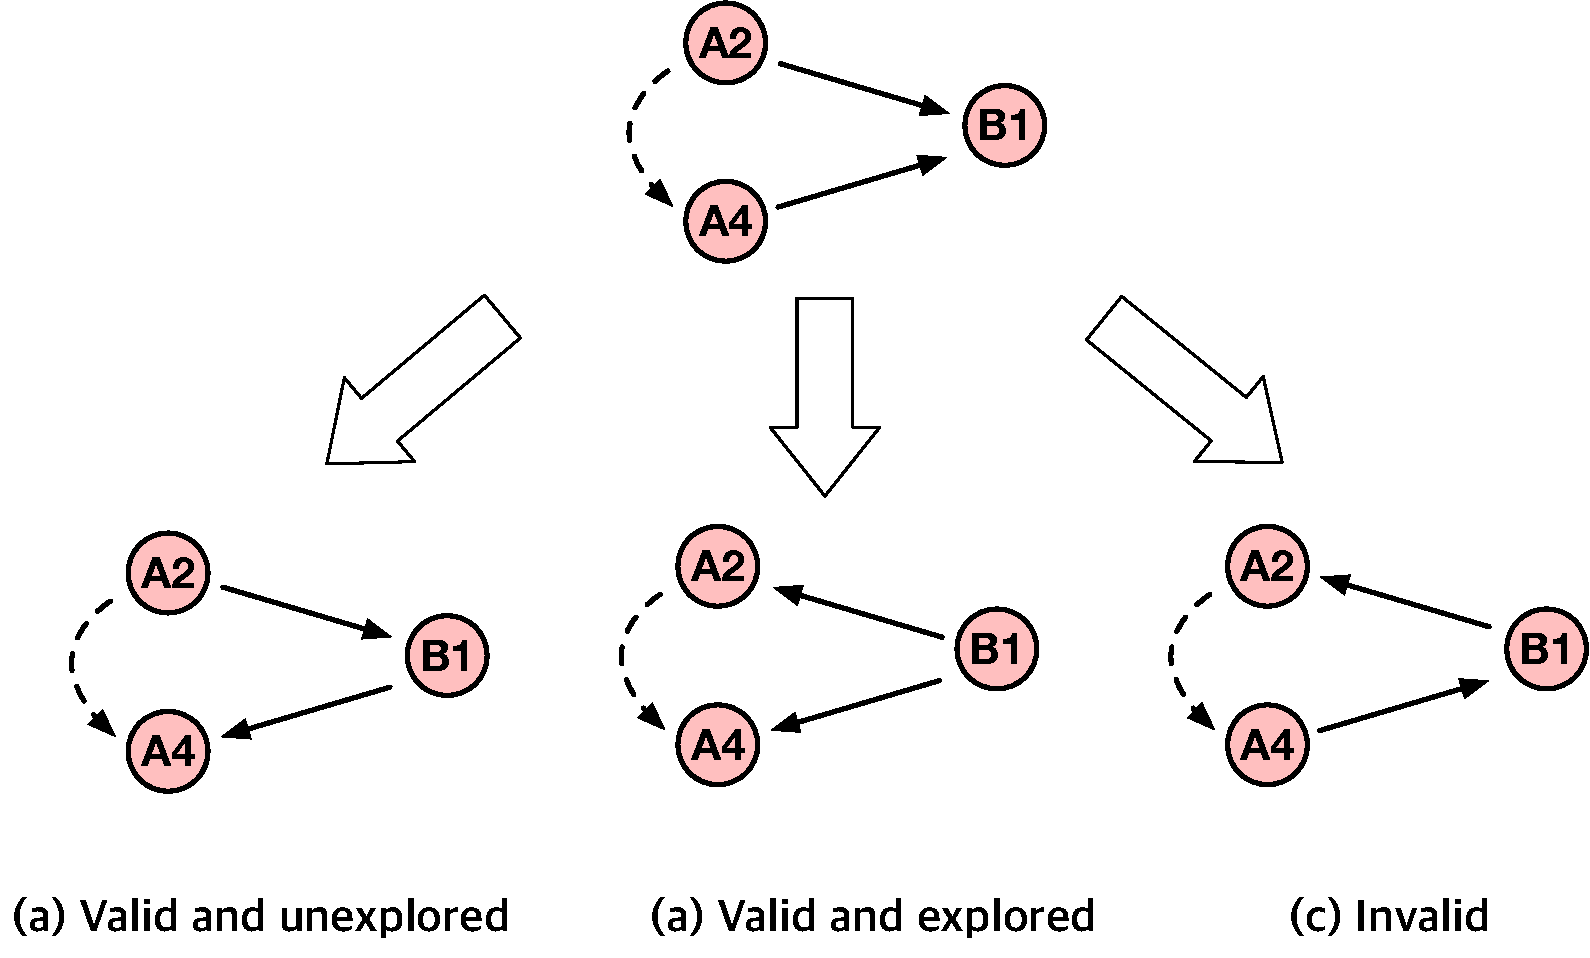
\includegraphics[width=0.7\linewidth]{fig/interleavingmutation.pdf}
  \caption{Example of interleaving segment mutation. In this example,
    (a) represents an interleaving segment graph of
    \autoref{fig:interleavingsegmentgraph} while (b) and (c) represent
    \textit{valid} mutated segments of (a). Whereas (d) is an
    \textit{invalid} mutated segment of (a) because it contains a
    loop.}
  \label{fig:interleavingmutation}
\end{figure}

\PP{Mutating interleaving segment}
%
% The first step is to derive \textit{unexplored} segment graphs from
% \textit{explored} segment graphs. We call this derivation operation
% \textit{mutating a segment graph}.
% %
Suppose a set of \textit{explored} segment graphs
$G = \{g_1, g_2, ..., g_n \}$ (\eg, segment graphs corresponding to
\autoref{fig:keyidea}-(b)) is given.
%
For each $g_i \in G$, a fuzzer mutates $g_i$ by flipping the
directions of its interleaving-order edges, which implies changing the
interleaving order of an instruction pair that access the same memory
object.
%
\autoref{fig:interleavingmutation} illustrates how a fuzzer mutates a
segment graph.
%
Given an explored segment graph described in
\autoref{fig:interleavingmutation}-(a), flipping
($\texttt{B1} \Rightarrow \texttt{A2}$) produces a segment graph
described in \autoref{fig:interleavingmutation}-(b).
%
%In \autoref{fig:interleavingmutation}-(a), an edge
%($\texttt{B1} \Rightarrow \texttt{A2}$) describes that
%``\textit{\texttt{B1} is executed before \texttt{A2}}'', while in
%\autoref{fig:interleavingmutation}-(b), an edge (\ie,
%$\texttt{A2} \Rightarrow \texttt{B1}$) describes that
%``\textit{\texttt{A2} is executed before \texttt{B1}}''.
%
Likewise, flipping both $(\texttt{B1} \Rightarrow \texttt{A2})$ and
$(\texttt{B1} \Rightarrow \texttt{A4})$ in
\autoref{fig:interleavingmutation}-(a) generates a different segment graph
of \autoref{fig:interleavingmutation}-(c), which also represents
another interleaving.
%
Note that flipping only
$(\texttt{B1} \Rightarrow \texttt{A4})$  of
\autoref{fig:interleavingmutation}-(a) generates an \textit{invalid}
segment graph as shown in \autoref{fig:interleavingmutation}-(d)
because it creates a loop
$\texttt{B1} \Rightarrow \texttt{A2} \Rightarrow \texttt{A4}
\Rightarrow \texttt{B1}$.
%
% \yj{cut if no space.
% Since edges represent execution orderings, a loop in a segment graph
% indicates a contradiction on the execution order, stating that any
% vertex on the loop should be executed before itself.}
%
When a mutated segment graph contains a loop, a fuzzer discards the
segment.
%
Also, a fuzzer drops a mutated segment graph if it is already
explored. A fuzzer identifies the case when the hash value of a newly
mutated segment graph is recorded in \intcov.
% In this way, a fuzzer generates mutated segment graphs of all
% $g_i \in G$, while excluding 1) invalid segment graphs (\ie, ones
% that contain a loop), and 2) explored segment graphs (\ie, ones that
% their hash values are recorded in the hash table).
%
In such way, a fuzzer forms a set of \textit{unexplored} mutated
segment graphs $G_{mutated}$, and recomposes them for the next search.
%
In the case of \autoref{fig:keyidea}, $G_{mutated}$ contains mutated
segment graphs (including \autoref{fig:interleavingmutation}-(b) and
(c)) derived from \texttt{Segment \#1}, \texttt{Segment \#2}, and
\texttt{Segment \#3}.

\PP{Recomposing mutated segment graphs}
%
One could take up a single mutated segment graph in $G_{mutated}$ for
the next search.
%
However, it might require many search iterations because the size of
$G_{mutated}$ could be large.
%
Instead, we select multiple mutated segment graphs in $G_{mutated}$,
and \textit{recompose} them to form a large graph to test multiple
mutated segments at one execution.
%
% \yj{briefly discuss the benefit over previous work?}

% choose a more efficient way. We \textit{recompose} a new
% thread interleaving from $G^*_{mutated} \subseteq G_{mutated}$, and by
% running the recomposed thread interleaving, we test multiple unexlored
% segment mutations in $G^*_{mutated}$ at once.

\begin{figure}[t]
  \centering
  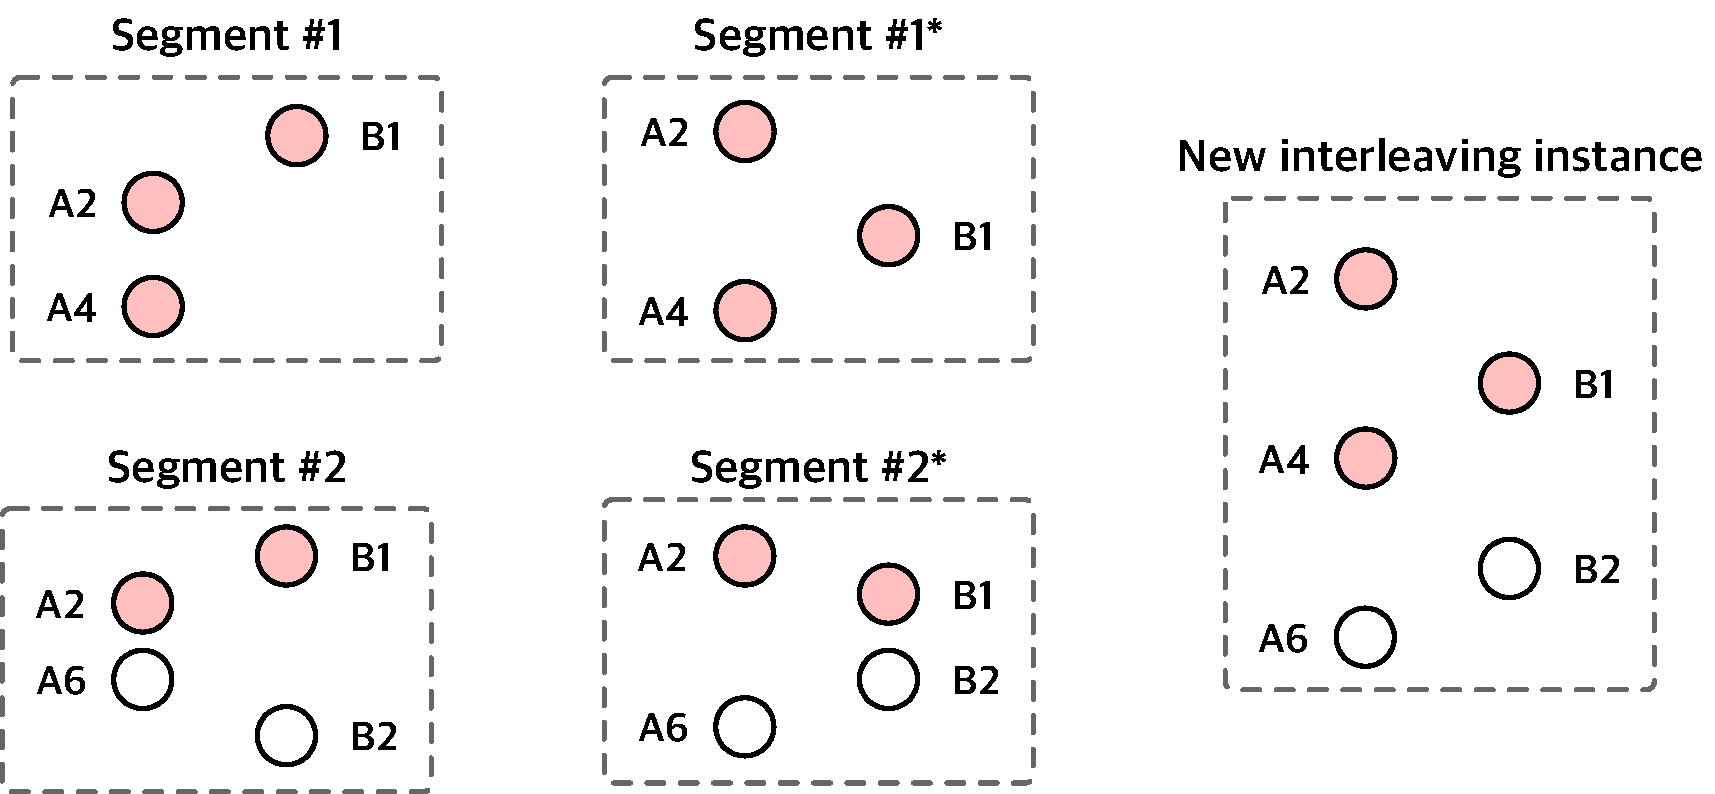
\includegraphics[width=\linewidth]{fig/hint.pdf}
  \caption{Example of recomposing mutated segments into whole
    interleaving. (a) represents mutated segments, (b) represents a
    graph combining the two mutated segments, and (c) represents a
    sequence of instructions to test \texttt{Segment \#1*} and
    \texttt{Segment \#2*}}
  \label{fig:hint}
\end{figure}


\autoref{fig:hint} demonstrates a sketch of recomposing steps. Suppose
we choose two mutated segment graphs from $G_{mutated}$ called
\texttt{Segment \#1*} and \texttt{Segment \#2*} (\ie,
\autoref{fig:hint}-(a)) that are derived from \texttt{Segment \#1} and
\texttt{Segment \#2} in \autoref{fig:keyidea}-(b) respectively.
%
We can then merge the two segment graphs, resulting in a
larger graph containing all vertices and all edges from \texttt{Segment
  \#1*} and \texttt{Segment \#2*} as described in
\autoref{fig:hint}-(b).
%
%In \autoref{fig:hint}-(b), five vertices are represented, where each
%vertex comes from either \texttt{Segment \#1*} or \texttt{Segment
  %\#2*}. It is worth noting that both segment graphs contain
%\texttt{A1} and \texttt{B1}, and only one copy is represented for each
%of them.
%
%Then, edges of \texttt{Segment \#1*} and \texttt{Segment \#2*} are
%also added into the merged graph.
%
%Similar to the vertex case, an edge
%($\texttt{A2} \Rightarrow \texttt{B1}$) is contained in both segment
%graphs, and only one copy of the edge is added.
%
%\dr{}
%
Therefore, when we execute instruction interleavings corresponding to this
large graph, we can test both \texttt{Segment \#1*} and \texttt{Segment
  \#2*} at once (\autoref{fig:hint}-(c)).

When recomposing mutated segment graphs, one important constraint is
that it should not contain a loop (\ie, \autoref{fig:hint}-(b) should
not contain a loop). 
%Otherwise, a contradiction on the execution order
%arises similar with an invalid mutation (\ie, an instruction should be
%executed before itself).
%
To select a subset $G^*_{mutated}$ without making a loop, we start
with an empty set of $G^*_{mutated}$. Then, we iterate over mutated
segment graphs in $g^* \in G_{mutated}$ where $g^*$ is a mutated
segment graph of a segment graph $g$.  From $g^*$, we try to add edges
in $g^*$ into $G^*_{mutated}$ one by one and check it causes a loop or
not. If it does not form a loop, we add the segment graph $g^*$ into
$G^*_{mutated}$.
%
After iterating all mutated segment graphs in $G_{mutated}$,
a fuzzer obtains $G^*_{mutated}$ not containing a loop. Then, 
the fuzzer excludes selected mutated segment graphs from the set of 
all mutated segment graphs
(\ie, $G_{mutated} = G_{mutated} \setminus G^*_{mutated}$), and
generates scheduling points to execute instruction orders 
specified in $G^*_{mutated}$.


\PP{Generating scheduling points}
%
As a final step, once $G^{*}_{mutated}$ (\ie, \autoref{fig:hint}-(b))
is obtained, a fuzzer creates scheduling points, where each scheduling
point describes an instruction on which preemption should occur
(including the end of each system call) and the next thread to run.
%
% How to enforce a schedule point is described in \autoref{ss:engine}.
%In this sequence, scheduling points are just instructions that the
%preemption should happen; \ie, the next instruction is executed by a
%different thread.
A fuzzer generates scheduling points by conducting a topological
sort~\cite{topologicalsort} to $G^{*}_{mutated}$, which generates a
sequence of instructions to run.
%
% Since $G^{*}_{mutated}$ is acyclic, a topological sort
% always returns a sequence of vertices (\ie, instructions) that does
% not violate a program order.
% %
\autoref{fig:hint}-(c) shows the result of conducting the topological
sort to \autoref{fig:hint}-(b).
%
As shown in the figure, a fuzzer can obtain the sequence of
instructions to test mutated segments \texttt{Segment \#1*} and
\texttt{Segment \#2*}. In this instruction sequence, a fuzzer selects
scheduling points as \texttt{A2}, \texttt{B2} and \texttt{A6}, and
uses scheduling points when enforcing thread scheduling as detailed in
\autoref{ss:engine}.


%
% \dr{I wrote the time complexity when writing the first draft. Do we
%   need it?}
% %
% It is well known that the time complexity of a topological sort is
% $O(V+E)$. Considering that the graph is sparse, $E$ is a small value
% so the time complexity can be asymptotically considered as $O(V)$.
%




%%% Local Variables:
%%% mode: latex
%%% TeX-master: "p"
%%% End:
